\subsection[Extractor]{Extractor \myAuthor{Simon Hampp}} \label{sec:extractor}

\subsubsection{Motivation}
Zu lösen war das Extrahieren der Kanten aus den PNG der Puzzleteile. Die Puzzleteile sind alle einzeln abfotografiert, schon segmentiert und optisch korrigiert.

Die Annahme ist also, dass der Alphakanal Vorder- und Hintergrund voneinander trennt und kein zusätzliches Preprocessing des PNG mehr nötig ist.

Um das Puzzle zu lösen, braucht man jedoch mehr als nur die optische Darstellung. Das Ziel ist es, anhand des Bildes alle vier Kanten zu extrahieren, und für jede Kante einen eindeutigen Pfad zu extrahieren, sowie den Typ der Kante. Wir unterscheiden zwischen $female, male, flat$ Kanten.

\subsubsection{Vorgehen}
Zuerst wird die gesamte Kante des Puzzleteils extrahiert und dann die Kante an den vier Ecken des Puzzles geteilt. Im letzten Schritt wird der Verlauf der jeweiligen Kante analysiert, um herauszufinden, um welchen Typ es sich handelt.

Der erste Schritt ist trivial, da der Alpha-Kanal des PNG schon die Kante repräsentiert. Die erste Pixelreihe, die nicht mehr transparent ist, ist die Kante des Puzzles.

Der nächste Schritt, die Ecken zu finden, ist das schwierige. Hierfür habe ich recherchiert, welche bestehenden Methoden existieren und insbesondere welche Methoden OpenCV bereitstellt, um es in Python zu implementieren. Ich habe mehrere Methoden hierfür ausprobiert, wie bspw. Hough Transformation, goodFeaturesToTrack und Harris Corner Detection. Hierbei gab es jedoch das Problem, dass die Methoden einzeln entweder nicht die richtigen vier Ecken zuverlässig gefunden haben oder zu unpräzise waren. Vor allem mit der Hough Transformation konnten nicht alle Ecken finden, da diese Methode oft nur lokal in spezifischen Regionen der Kante Geraden angelegt hat.
Nur goodFeaturesToTrack() von OpenCV konnte zuverlässig die vier Ecken der Puzzleteile finden, jedoch waren diese zu unpräzise. Die gefundenen Ecken liegen nicht direkt auf der Kante, sondern etwas näher im Inneren, wie auch in \autoref{fig:hough_zoom} zu erkennen.

\subsubsection{Lösung}
\paragraph{Kanten extrahieren}
Um Ecken zuverlässig und präzise zu erkennen, wurde eine Kombination aus goodFeaturesToTrack und Hough Transformation gewählt. Mit goodFeaturesToTrack werden die Regionen der vier Ecken gefunden, und in diesen Regionen die Hough Transformation lokal angewendet. Bei der Hough Transformation ist zusätzlich noch zu beachten, dass eine Fallbacklogik eingebaut ist; sollten die beiden besten Geraden nicht plausibel sein, werden immer mehr Gerade gesucht, bis eine Kombination aus zwei plausiblen Geraden gefunden wird. Plausible Geraden sind definiert als zwei Geraden, die einen Winkel aufspannen, der größer als 45 Grad und kleiner als 135 Grad. Mit dieser Einschränkung findet der Extractor für alle 49 Puzzleteile in unserem Beispiel Puzzle die richtigen Ecken.

In Algorithmus \ref{alg:edge_extraction} ist nochmal der schematische Ablauf der Kanten-Extraktion abgebildet.

\begin{algorithm}

\caption{Kantenextraktion aus einem PNG-Bild}\label{alg:edge_extraction}
\begin{algorithmic}[1]
\State \textbf{Eingabe:} PNG-Bild $\text{image}$
\State \textbf{Ausgabe:} Liste von Kanten $\text{edges}$

\State $\text{edge} \gets \text{GetEdgeUsingAlphaChannell(png)}$
\State $\text{corners} \gets \text{GoodFeaturesToTrackOpenCV}(\text{edge})$
\State $\text{final\_corners} \gets \text{[]}$
\For{$\text{corner} \in \text{corners}$}
    \State $\text{corner\_region} \gets \text{GetCornerRegion(edge, corner)}$
    \State $\text{line}_1 \text{ and } \text{line}_2 \gets \text{GenerateLinesWithHoughTransformation}(\text{corner\_region})$
    \State $\text{intersection} \gets \text{CalculateIntersection}(\text{line}_1, \text{line}_2)$
    \State $\text{nearest\_point} \gets \text{GetNearestPointOnEdge(edge, intersection)}$
    \State \text{Füge } $\text{nearest\_point}$ \text{ zu } $\text{final\_corners}$ \text{ hinzu}
\EndFor
\State $\text{edges} \gets \text{SplitEdgeAtCorners(final\_corners, edge)}$
\State \Return $\text{edges}$
\end{algorithmic}

\end{algorithm}


Wie die Extrahierung in der Praxis aussieht, ist an \autoref{fig:hough_input}, \autoref{fig:hough_output}, \autoref{fig:hough_zoom} zu erkennen. In \autoref{fig:hough_input} ist der Input der Hough Transformation abgebildet, im Algorithmus \ref{alg:edge_extraction} entspricht dies der $corner\_region$. In \autoref{fig:hough_output} sieht man die Hough Geraden ($line_1, line_2$) geplottet auf dem Kantenbild ($edge$) des Puzzles. \autoref{fig:hough_zoom}, ist dasselbe wie \autoref{fig:hough_output} nur an die untere linke Ecke rangezoomt. So kann man den Schnittpunkt ($intersection$) und die Ecke, die goodFeaturesToTrack erkannt hat ($corner$), besser erkennen. Der grüne Punkt im Bild ist die endgültige Ecke, die den nächsten Punkt ($nearest\_point$) auf der Kante zu dem Schnittpunkt darstellt, gemessen anhand der Euklidischen Distanz.

\begin{figure}[h!]
    \centering
    \begin{minipage}[b]{0.3\textwidth}
        \centering
        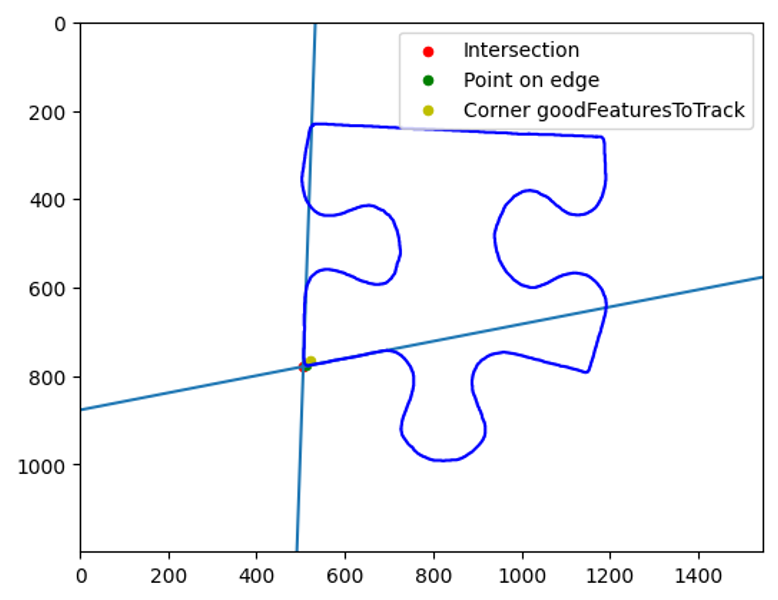
\includegraphics[width=\textwidth]{sections/solver/images/hough.png}
        \caption{Input für Hough Transformation}
        \label{fig:hough_input}
    \end{minipage}
    \hfill
    \begin{minipage}[b]{0.3\textwidth}
        \centering
        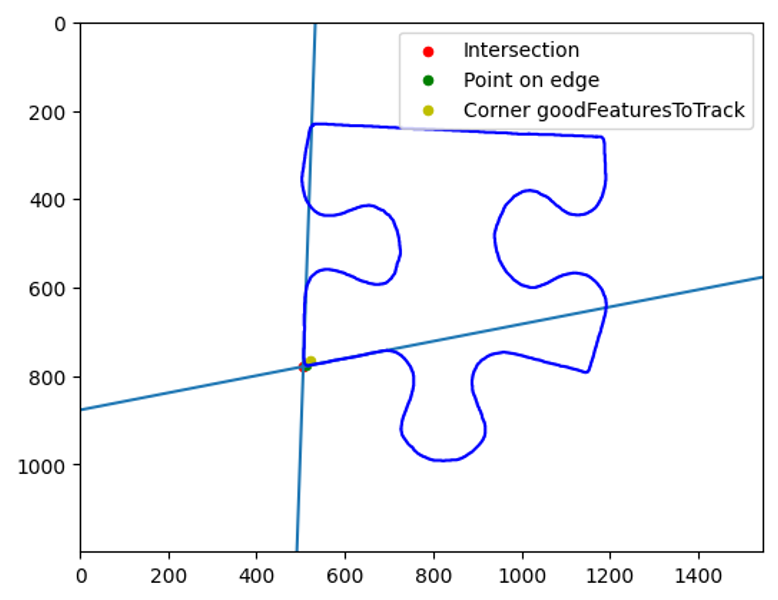
\includegraphics[width=\textwidth]{sections/solver/images/hough.png}
        \caption{Output Hough Transformation}
        \label{fig:hough_output}
    \end{minipage}
    \hfill
    \begin{minipage}[b]{0.3\textwidth}
        \centering
        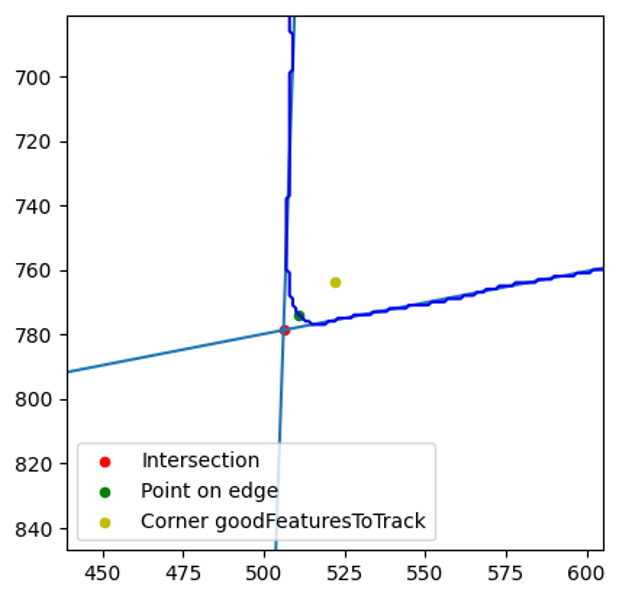
\includegraphics[width=\textwidth]{sections/solver/images/hough_zoomed.png}
        \caption{Zoom an Ecke}
        \label{fig:hough_zoom}
    \end{minipage}
\end{figure}


\paragraph{Kantentyp}

\begin{figure}[h!]
    \centering
    \begin{minipage}[b]{0.4\textwidth}
        \centering
        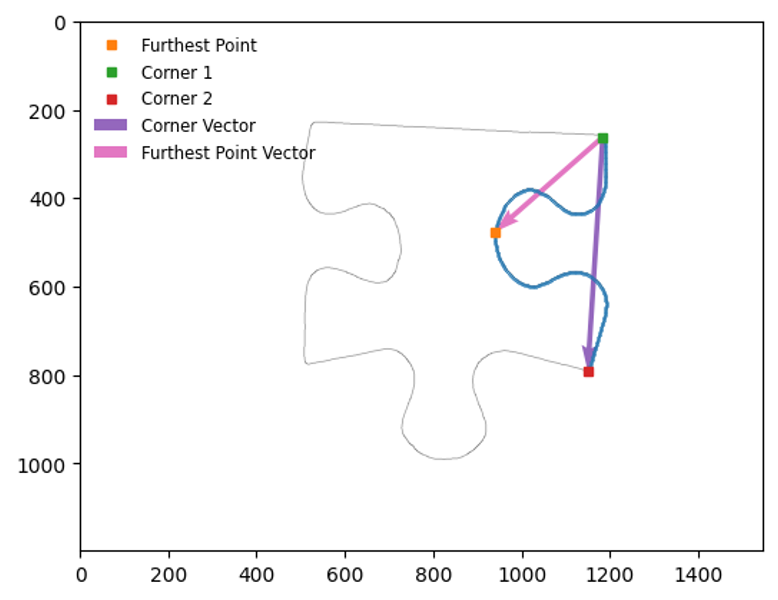
\includegraphics[width=\textwidth]{sections/solver/images/edge_type.png}
        \caption{Kantentyp: $female$}
        \label{fig:edge_type_female}
    \end{minipage}
    \hfill
    \begin{minipage}[b]{0.4\textwidth}
        \centering
        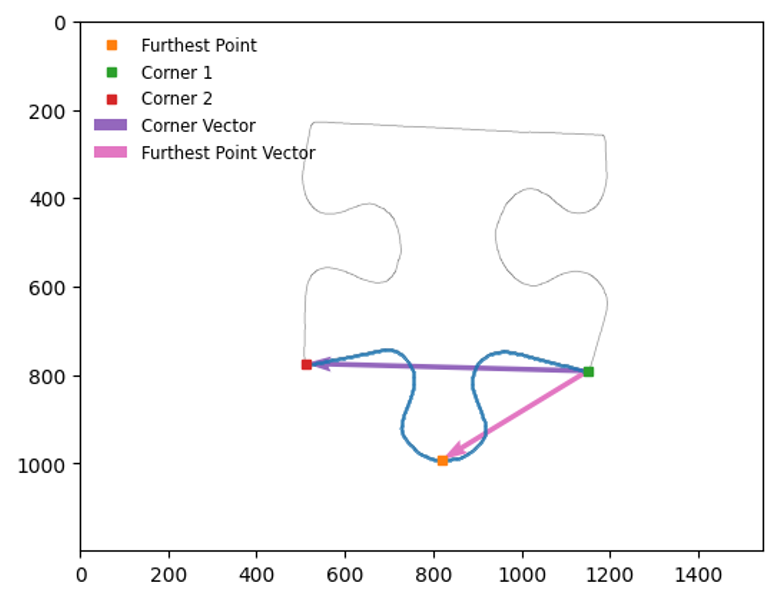
\includegraphics[width=\textwidth]{sections/solver/images/edge_type_1.png}
        \caption{Kantentyp: $male$}
        \label{fig:edge_type_male}
    \end{minipage}
    \hfill
\end{figure}

Anhand der gefundenen Kanten und Ecken muss im letzten Schritt noch der Typ ($male, female, flat$) der Kante erfasst werden. Im Code hat die Kantenklasse einen Pfad, der einem numpy Array entspricht, der die 2D-Koordinaten der Kante speichert. Der Kantentyp muss anhand dieses Pfads und der zwei Ecken, die die Kante aufspannt, erkannt werden. Hierfür wurde ein CCW Test implementiert. Bei der Implementierung der Kanten-Extraktion wurden alle Kanten und deren Ecken im Uhrzeigersinn (CW) definiert und so auch in den Datentypen abgespeichert. Diese Orientierung kann nun genutzt werden. Ein Vektor wird aufgespannt von der ersten bis zur nächsten Ecke. Dann ein weiterer Vektor von der ersten Ecke bis zu dem Punkt auf dem Kantenpfad, der am weitesten vom Vektor der Ecken entfernt ist. Anschließend wird geprüft, ob der Vektor zum weitesten Punkt links oder rechts vom Ecken-Vektor ist. Ist er links, ist es eine Kante vom Typ $male$. Ist der Vektor recht, ist die Kante vom Typ $female$. Zuletzt wird noch überprüft, wie weit der Punkt vom Vektor entfernt ist; ist die Entfernung sehr klein, wird der Typ auf $flat$ gesetzt. Den Threshold, ab wann eine Kante $flat$ ist, ist empirisch ermittelt worden. Übliche Werte der maximalen Distanz eines Kantenpunkts zum Ecken Vektor für nicht $flat$ sind in der Größenordnung $10^2$, wohingegen Werte für $flat$ in der Größenordnung $10^0$ liegt. Deshalb lassen sich diese Typen sehr gut voneinander unterscheiden.

